

\subsection{Colocation Factor}
\label{eval-colo}


% \hsg{Form this story in another way: Scalable Testing, and then Scalable
% Replay.}

% \hsg{Does the unit test scalable enough to do scale test? apparent NO NO
% ... lots of thread context switching ... }

% \hsg{Can we prevent context switching with a lock??}






We first show the maximum colocation factor \sck can achieve as each
technique is added {\em one at a time} on top of the other.  To recap, the
techniques are: 
single-process cluster (SPC; \sec\ref{sc-spc}), 
memory footprint reduction (MFR; \sec\ref{sc-mfr}),
global event driven architecture (GEDA; \sec\ref{sc-geda}), and 
processing illusion (PIL; \sec\ref{sc-pil}).
%
The results are based on a 16-core machine.
%machine \cite{NomeNodes}.


% \hsg{show even lateness just by increasing nodes }

% define maximum colocation factor
\vni {\bf Maximum colocation factor (``MaxCF''):} A maximum colocation factor
is reached when the target system's behavior in \sck mode starts to
deviate from the real deployment behavior.
%
Deviation happens when one or more of the following bottlenecks are
reached:
%
(1) high average CPU utilization ($>$90\%),
%
(2) memory exhaustion (nodes receive out-of-memory exceptions and crash), and
%
(3) high event ``lateness''; 
queuing delays from thread context switching can make events late to be 
processed,
although CPU utilization is not high.
%
We instrument our target systems to measure {\em event lateness} of
relevant events (\eg, gossip sending, gossip processing, and failure
detection events).  For example, if gossips should be sent every 1 second,
but they are sent every 1.5 second on average, then the lateness is 50\%.
%
We use 10\% as the maximum acceptable event lateness.
%
Note that the residual limiting bottlenecks above come from the main logic
of the target protocols, which cannot be removed with general methods.


% figures
\vni {\bf Results and observations:} Figure \ref{fig-colo} shows {\em
  different sequences of integration} to our four target systems and the
resulting maximum colocation factors.  We discuss four important findings
from this figure.

% ..
First, when multiple techniques are combined, they collectively achieve a
high colocation factor (up to 512 nodes for the three
systems respectively).
%
For example, in Figure \ref{fig-colo}a, with just adding SPC+GEDA to
Cassandra, MaxCF only reaches 136.  But with SPC+GEDA+PIL, MaxCF
significantly jumps to 512.
%
When we increase the colocation factor (+100 nodes) beyond the maximum, we
hit the residual bottlenecks mentioned before; at this point, we do not
measure MaxCF with small increments (\eg, +1 node) as pre-memoization takes
time.
%
The bug in Voldemort's rebalancing protocol involves sequential
operations (no parallel CPU-intensive computations), hence GEDA and PIL
are not necessary.  HDFS needs GEDA, but not PIL (the datanodes are not
CPU-intensive, only the master is)

%We will add GEDA and PIL to test Voldemort's latest
%stable code which involves parallel rebalancing.





\def \fgw {3in}


\begin{figure}[t]

\centerline{
\hspace{1.6cm}
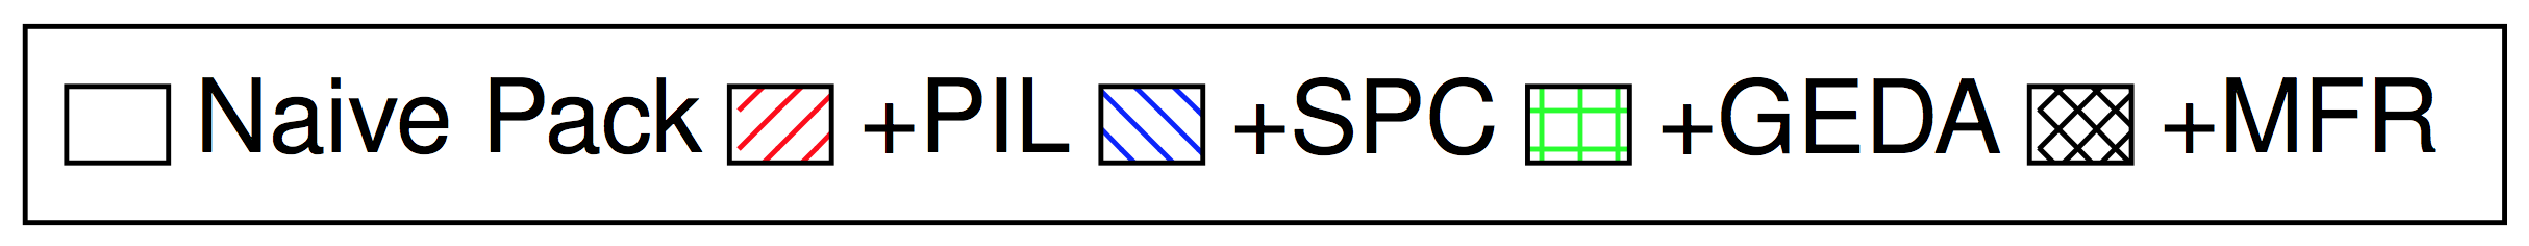
\includegraphics[width=2.5in]{F/colo/legend}
}
\centerline{

\begin{tikzpicture}[font=\sffamily\footnotesize]
\begin{axis}[
xbar stacked,
y=0.8cm,
width=\columnwidth,
xmin=0, xmax=512,
bar width=12pt,
symbolic y coords={VOLD, RIAK, CASS2, CASS1},
ytick=data,
yticklabels={{(d) Voldemort, (c) Riak, (b) Cass-2, (a) Cass-1}},
every axis y label/.style={at={(ticklabel cs:0.5)},rotate=90,anchor=near ticklabel},
axis y line*=left,
enlarge y limits={0.25},
legend style={at={(0.5,1.3)},anchor=north,legend columns=-1},
xmajorgrids=true,
xlabel=\#Nodes
]
\addplot [fill=white] plot coordinates {(80,VOLD) (16,RIAK) (48,CASS2) (48,CASS1)}; %mpc
\addplot [pattern=north east lines, pattern color=red] plot coordinates {(0,VOLD) (0,RIAK) (12,CASS2) (0,CASS1)}; %+pil
\addplot [pattern=north west lines, pattern color=blue] plot coordinates {(140,VOLD) (0,RIAK) (4,CASS2) (72,CASS1)}; %+spc
\addplot [pattern=grid, pattern color=green] plot coordinates {(0,VOLD) (0,RIAK) (448,CASS2) (16,CASS1)}; %+geda
\addplot [pattern=crosshatch, pattern color=black] plot coordinates {(292,VOLD) (48,RIAK) (0,CASS2) (0,CASS1)}; %+lma
\addplot [pattern=north east lines, pattern color=red] plot coordinates {(0,VOLD) (192,RIAK) (0,CASS2) (376,CASS1)}; %+pil
\addplot [pattern=north west lines, pattern color=blue] plot coordinates {(0,VOLD) (256,RIAK) (0,CASS2) (0,CASS1)}; %+spc
%\legend{Naive Pack,+PIL,+SPC,+GEDA,+MFR}
\end{axis}
\end{tikzpicture}

\if
Cassandra1
MPC: 48
SPC: 120 (+72)
SPC + GEDA: 136 (+16)
SPC + GEDA + PIL: 512 (+376)

Cassandra2
MPC: 48
PIL: 60 (+12)
PIL + SPC: 64 (+4)
PIL + SPC + GEDA: 512 (+448)
All: 512

Riak1
MPC: 16
LMA: 64 (+40)
LMA + PIL: 256 (+192)
SPC + LMA + PIL: 512 (+256)

Voldemort1
MPC: 80
SPC: 220 (+140)
MFR: 512 (+292)
\fi

}
\mycaption{fig-colo}{Maximum colocation factor (\sec\ref{eval-colo})}{}


\end{figure}


\if 0
\hsg{RIAK: find the final value., 
VOLD: how to speed up experiment time?? 
still waiting for network bypass??}
\fi


% independent
Second, distributed systems are implemented in different ways.
Thus, integrations to different systems face different sequences of
bottleneck.  To show this, we tried different {\em integration sequences}.
For example, 
%for reproducing \caone 
in Cassandra (Figure \ref{fig-colo}a),
our integration sequence is: +SPC, +GEDA, and +PIL (as we continuously hit
CPU contention).
%
For Riak (Figure \ref{fig-colo}c), we began with MFR as we hit
a memory bottleneck first (the excessive Erlang processes;
\sec\ref{sc-mfr}).
%\voldone in 
For Voldemort and HDFS (Figure \ref{fig-colo}d-e), we began with SPC to
reduce Java VM memory overhead.



Third, not all features get the chance to show their benefits, as the
fundamental bottlenecks are reached.  For example, for Cassandra and HDFS
(Figures \ref{fig-colo}a-c), MFR is unnecessary as we will hit CPU
contention in $>$512 nodes.  For Riak (Figure \ref{fig-colo}c),
GEDA is not needed as we will hit a memory bottleneck in $>$512 nodes, and
similarly for Voldemort (Figure \ref{fig-colo}d).




% showing its full potential
Fourth, an \sck technique can hit a different bottleneck before showing
its full potential.  For example, for Cassandra, we tried two different
integration sequences (Figure \ref{fig-colo}a-b).  With Naive Packing
(\sec\ref{sc-np}), we initially hit a MaxCF of 48 nodes due to CPU
contention.  At this point, there are two choices: add SPC+GEDA (to reduce
process/thread context switching) or PIL (to reduce expensive processing).
In Figure \ref{fig-colo}b, we tried +PIL first and we found that it does
not help much as process/thread queuing delays are still the bottleneck.
Similarly, in Figure \ref{fig-colo}a, SPC+GEDA also can only reach a
certain maximum.  This again highlights that it is the {\em combination}
of the techniques that make \sck powerful.

